% The figure belonging to §5. Held in its own file so main.tex and review_s5.tex share one
% copy and the export cannot drift from the manuscript.
\begin{figure}[t]
  \centering
  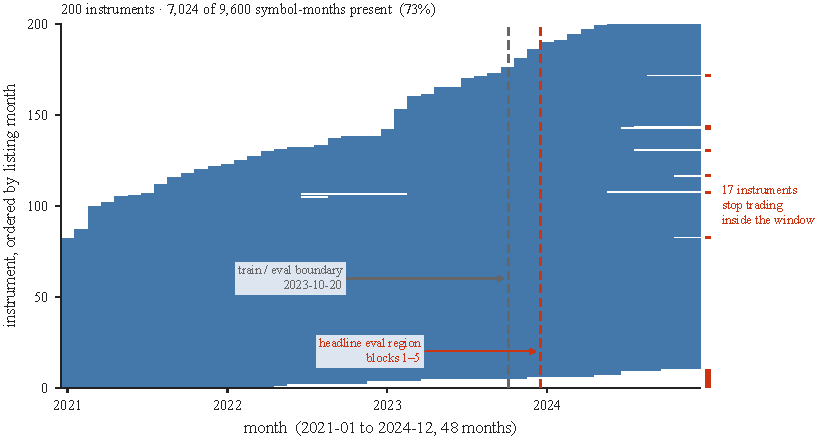
\includegraphics[width=\textwidth]{figures/fig7_coverage.pdf}
  \caption{\textbf{Survivorship is owned, not filtered away.} Month-by-month presence for all $200$
  instruments over the four-year window, ordered by listing month: $7{,}024$ of a possible
  $9{,}600$ symbol-months are present. The left staircase is instruments listing at different
  times; the right edge is ragged because instruments that stop trading are \emph{kept}, and $17$
  of them stop inside this window. A survivorship-filtered universe would render as a solid
  rectangle, which is the artefact this panel exists to show we did not create. Two instruments
  have interior gaps rather than truncated tails and appear as internal white streaks. The two
  dashed rules are the committed fold plan: training ends at the first, and the headline metric is
  scored only to the right of the second. Note that $17$ counts instruments whose data ends inside
  the window; the ingest record's $41$ counts every instrument known to be delisted at any date,
  including $24$ that delist after this window closes.}
  \label{fig:coverage}
\end{figure}
